\documentclass[journal=jctcce,manuscript=article]{achemso}
\usepackage{amsmath,amssymb,xspace}
\usepackage{hyperref}

\newcommand{\numpy}{{\sc{NumPy}}\xspace}%
\newcommand{\pfour}{{\sc{Psi4}}\xspace}%
\newcommand{\pfn}{{\sc{Psi4NumPy}}\xspace}%

\title{\pfn: An Interactive Quantum Chemistry Programming Environment for Reference Implementations and Rapid Development}

\author{Daniel G. A. Smith}
\email{dgasmith@gatech.edu}
\author{Lori A. Burns}
\author{Dominic A. Sirianni}
\affiliation{
    Center for Computational Molecular Science and Technology,
    School of Chemistry and Biochemistry,
    School of Computational Science and Engineering,
    Georgia Institute of Technology,
    Atlanta, Georgia 30332-0400, United States}

\author{Daniel R. Nascimento}
\affiliation{
    Department of Chemistry and Biochemistry,
    Florida State University,
    Tallahassee, Florida 32306-4390, United States}

\author{Ashutosh Kumar}
\author{Andrew M. James}
\affiliation{
    Department of Chemistry, Virginia Tech,
    Blacksburg, Virginia 24061, United States}

\author{Jeffrey B. Schriber}
\author{Tianyuan Zhang}
\affiliation{
    Department of Chemistry, Emory University,
    Atlanta, Georgia 30322, United States}

\author{Boyi Zhang}
\author{Adam S. Abbott}
\affiliation{
    Center for Computational Quantum Chemistry, University of Georgia,
    Athens, Georgia 30602, United States}

\author{Eric Berquist}
\affiliation{
    University of Pittsburgh, Pittsburgh, PA, 15260, United States}

\author{Marvin Lechner}
\affiliation{
    Department of Chemistry, Technical University of Munich, Munich, Germany}

\author{Leonardo dos Anjos Cunha}
\affiliation{
    The Technical Institute of Aeronautics, S\~{a}o Jos\'{e} dos Compos, Brazil}

\author{Alexander G. Heide}
\author{Rollin A. King}
\affiliation{
    Department of Chemistry, Bethel University, St. Paul, Minnesota 55112, United States}

\author{Andrew C. Simmonett}
\affiliation{
    National Institutes of Health -- National Heart, Lung and
    Blood Institute, Laboratory of Computational Biology,
    5635 Fishers Lane, T-900 Suite, Rockville, Maryland 20852, United States}
\author{Justin M. Turney}
\author{Henry F. Schaefer}
\affiliation{
    Center for Computational Quantum Chemistry, University of Georgia,
    Athens, Georgia 30602, United States}
\author{Francesco A. Evangelista}
\affiliation{
    Department of Chemistry, Emory University,
    Atlanta, Georgia 30322, United States}
\author{A. Eugene DePrince III}
\affiliation{
    Department of Chemistry and Biochemistry,
    Florida State University,
    Tallahassee, Florida 32306-4390, United States}
\author{T. Daniel Crawford}
\affiliation{
    Department of Chemistry, Virginia Tech,
    Blacksburg, Virginia 24061, United States}
\author{Konrad Patkowski}
\affiliation{
    Department of Chemistry and Biochemistry,
    Auburn University,
    Auburn, Alabama 36849, United States}
\author{C. David Sherrill}
\affiliation{
    Center for Computational Molecular Science and Technology,
    School of Chemistry and Biochemistry,
    School of Computational Science and Engineering,
    Georgia Institute of Technology,
    Atlanta, Georgia 30332-0400, United States}

\begin{document}

\begin{abstract}
  \pfn demonstrates the use of efficient computational kernels from the open-source \pfour program through the popular \numpy library for linear algebra in Python to facilitate the rapid development of clear, understandable Python computer code for new quantum chemical methods, while maintaining a relatively low execution time.  Using these tools, reference implementations have been created for a number of methods, including self-consistent field (SCF), SCF response, many-body perturbation theory, coupled-cluster theory, configuration interaction, and symmetry-adapted perturbation theory.  Further, several reference codes have been integrated into Jupyter notebooks, allowing background and explanatory information to be associated with the implementation.  \pfn tools and associated reference implementations can lower the barrier for future development of quantum chemistry methods.  These implementations also demonstrate the power of the hybrid C++/Python programming approach employed by the \pfour program.
\end{abstract}

\maketitle

\section{Introduction}

Whereas in the past a new quantum chemical (QC) method was commonly presented solely through its equations, perhaps along with a few token values, the more recent expectation is that equations will be accompanied by results from an effective computer program clearly demonstrating the utility of the method.  This expectation becomes increasingly burdensome as new computer architectures emerge, since some theories will be naturally more computationally efficient or more difficult to implement than others.  The computation expense of most quantum chemical methods creates substantial pressure for methods to be implemented with highly optimized algorithms.

This situation presents a challenge for ongoing development in quantum chemistry, because new theoretical methods are typically complex and their correct implementation is non-trivial.  Additionally, computationally efficient codes require a low-level programming language like C++ or Fortran, followed by substantial code profiling, testing, and optimization.  Often a method's first implementation is a rather messy computer program. The researcher may be learning the details of the method as they progress, resulting in ``experimental'' parts of the code that may never get removed, or data structures that may not be optimal for the final version of the method.  Additionally, development is often carried out by graduate students not yet proficient in programming, resulting in unconventional coding styles.  Subsequently, a researcher seeking to extend or enhance a method previously developed in-house is often faced with the daunting prospect of deciphering a quite complex existing code.

Still more challenging is implementing or extending an existing method sourced solely from the literature.  Often, a paper describing a new quantum chemical method that properly focuses on scientific detail falls short on algorithmic or numerical detail sufficient for independent reimplementation. Indeed, the methods are so complex that the original equations frequently include typos, which are generally tracked through institutional lore rather than published errata.  Additionally, modern approaches often employ combinations of approximations with multiple numerical cutoffs, exacerbating the reproducibility problem.  This paradigm is illustrated within a recent comment,\cite{Briling:2017:157101} whereby several corrections to equations originally published in 2011 for a two-level semi-empirical method\cite{Laikov:2011:134120} were proposed after being re-engineered to reproduce values computed using a binary program distributed with the original publication.  Even facilitated through private communication with the method's author, this cycle of rediscovery and reimplementation is both highly non-trivial and unsustainable.  Fortunately, an open-source program\cite{brilingqm} has been made available by the commenting author that implements the method and proposed changes, so that further extensions of the method can proceed with this program as a reference.

Such ``reference implementations'' (easy-to-read, unoptimized computer programs solely targeting the correct result) can be a helpful initial step toward developing or understanding a complex method, yet they are not widely available in quantum chemistry.  To our knowledge, reference implementations and benchmarking have only been performed in a large-scale way for density functional theory (DFT) exchange-correlation kernels\cite{CCL_DFT} and periodic boundary condition DFT with pseudopotentials.\cite{Lejaeghereaad3000} One factor limiting more widespread use of reference implementations for quantum chemistry is that methods are often so computationally demanding that a basic, unoptimized implementation is too slow for computations on even the smallest molecules.  What is needed is an alliance of QC code that is easy to peruse and manipulate with underlying non-QC routines that are fast enough for testing on non-trivial molecules.

Here we present \pfn, a framework for the creation of clear, readable reference implementations of quantum chemical methods and for the rapid development of new methods. \pfn takes advantage of \pfour's\cite{Psi41.1} application programming interface (API) that makes efficient computational kernels written in C++ available from Python, a language that is easy to learn and has become very popular in scientific computing.  As a high-level language, Python allows complex tasks to be specified with relatively few lines of code.  \pfn capitalizes on the straightforward conversion of \pfour tensors to \numpy\cite{Varoquaux:1521-9615} and Numerical Python's (\numpy's) own low-level back end to ensure that all data arrays can use the optimized Basic Linear Algebra Subroutines (BLAS) library\cite{BLAS} for common linear algebra operations. The wide user base of \numpy ensures constant updates and bug fixes. \pfn has been packaged for minimal setup, requiring only 3 minutes, with no preinstalled compilers necessary on 64-bit Linux, Mac, and Windows.  Here we introduce the main elements of the \pfn framework and illustrate them with a substantial collection of reference implementations for standard quantum chemical methods and numerical techniques. The \pfn is built entirely on Free and Open Source Software (FOSS)\cite{FOSS} as shown in Fig.~\ref{fig:ovalorg} to ensure a barrierless entry to quantum chemistry programming.

Several of the reference implementations have been augmented by tutorial-style introductions to the relevant theory.  The \pfn tutorial collection includes self-consistent field (SCF), DFT,\cite{Parr:1989} many-body perturbation theory (MBPT),\cite{Bartlett:1981:359} symmetry-adapted perturbation theory (SAPT)\cite{Jeziorski:1994:1887, Szalewicz:2012:254}, coupled-cluster (CC)\cite{Purvis:1982}, and configuration interaction (CI)\cite{Shavitt:1977,Sherrill:1999:CI} theories, with additional sections detailing the theory and implementation of linear response, geometry optimizations, and Verlet integrators.  It is our hope that \pfn and the accompanying reference code will lower the barrier to implementing quantum chemical methods.

\begin{figure}
  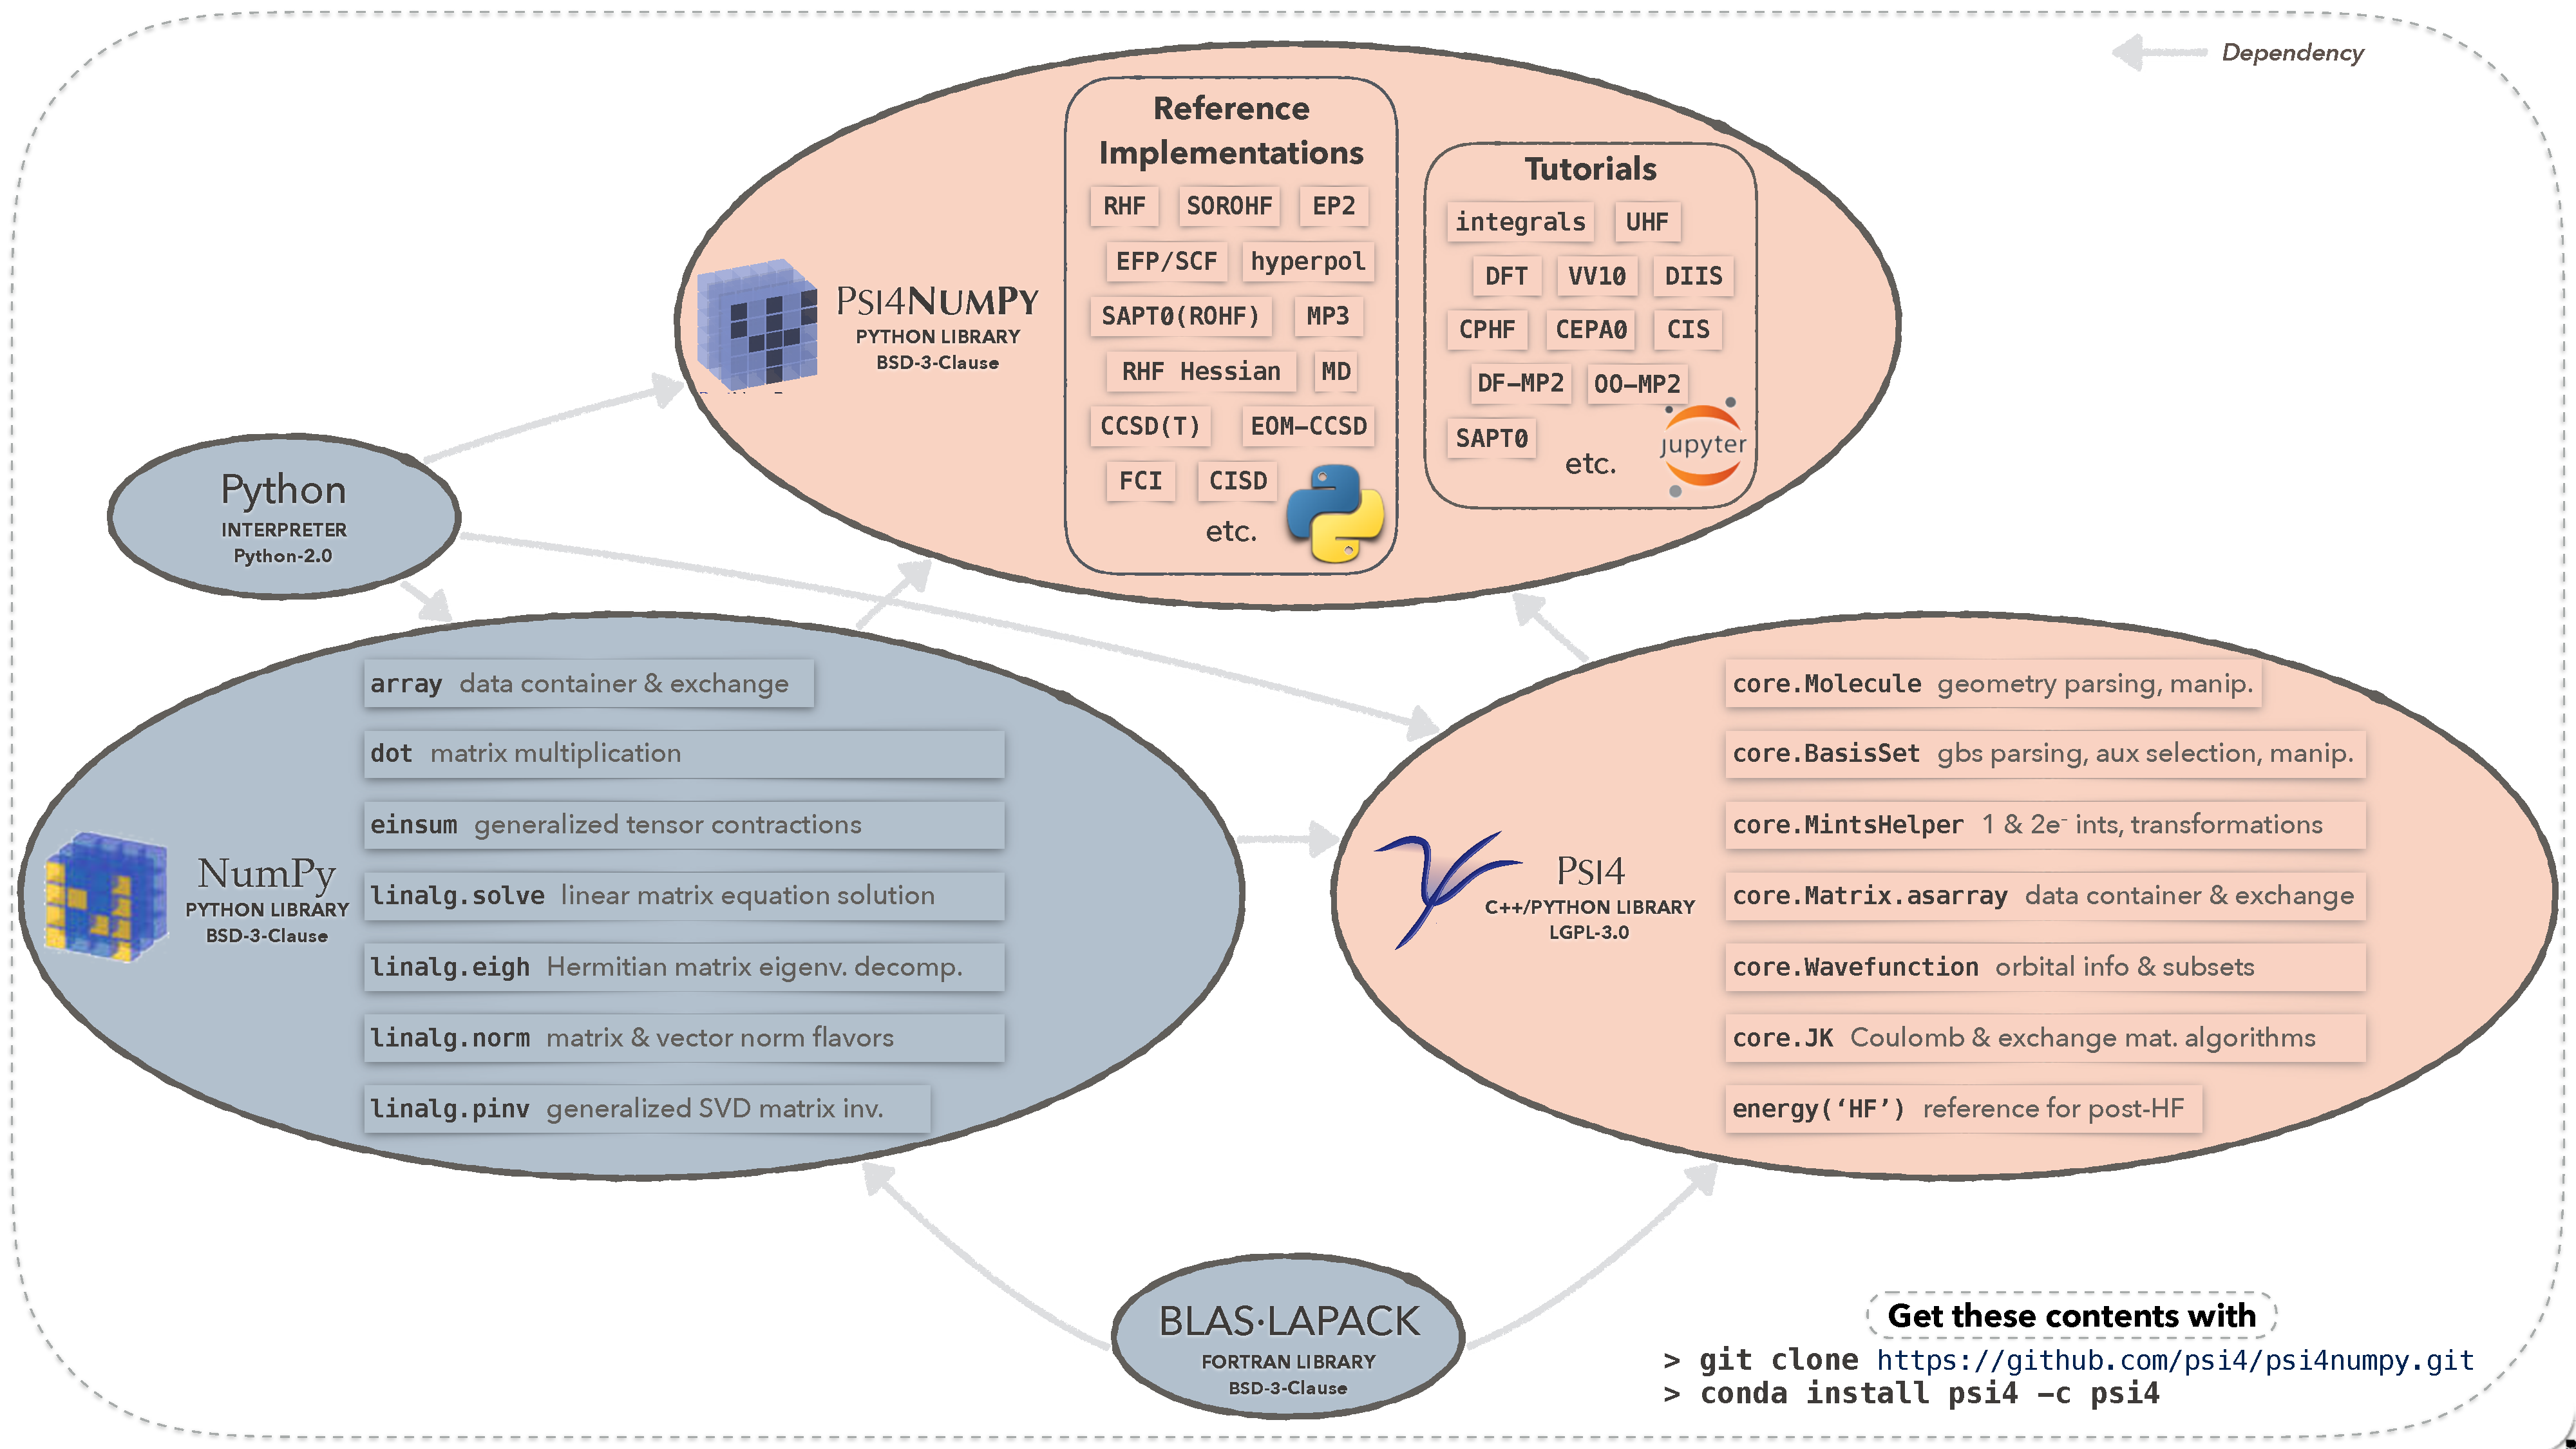
\includegraphics[width=\linewidth,keepaspectratio]{fig1-oval-org.pdf}
  \caption{\pfn draws linear algebra tools from \numpy and fundamental quantum chemistry structures from \pfour to bring together a practical and convenient environment for code development, verification, and exploration. The most important data structures and functions are shown for \numpy and \pfour as well as representative tutorial and reference implementations presently in \pfn.\label{fig:ovalorg}}
\end{figure}

Shortly before submission, the authors chanced upon the Quantum Chemistry Program Exchange (QCPE)\cite{QCPE, Boyd:2013:221}, whose goals of software (particularly self-contained software) accessibility, algorithm explication, and free software ``publishing'' \pfn shares. The general tools embraced by \pfn (GitHub for communication, \numpy for linear algebra, Python for interfacing, and Jupyter for illumination) further allow rapid prototyping and educational objectives. In this manner \pfn can be thought as a modern successor to QCPE built to serve the flexible needs of the community.

\section{Basic Tools}

The basic premise of \pfn is to leverage \pfour to generate quantum chemistry-specific quantities and the \numpy library\cite{Varoquaux:1521-9615} for all other tensor manipulations.  The latest version of \pfour has added the capability to import \pfour as a Python module as well as continuing to be called in an executable fashion. In this way, both the \pfour and \numpy libraries can be loaded into a single Python script and used in cooperation.

A key capacity in this enterprise is seamless translation between \numpy and \pfour data classes. For example, converting from a \numpy array to a \pfour matrix and back again can be easily accomplished:
\begin{eqnarray}
  \begin{aligned}
    &\verb!import numpy, psi4! \\[-10pt]
    &\verb!np_array = numpy.zeros((5, 5))! \\[-10pt]
    &\verb!psi4_matrix = psi4.core.Matrix.from_array(np_array)! \\[-10pt]
    &\verb!new_np_array = numpy.array(psi4_matrix)! \\[-10pt]
  \end{aligned}
  \label{snip:np2p42np}
\end{eqnarray}
%Refer as Eq.~\ref{snip:np2p42np}.
At the core of this procedure is \textsc{NumPy}'s {\tt array\_interface}\cite{array_interface} protocol, a basic specification for dense matrices consisting of
\begin{enumerate}
\item (a) the starting memory location for an in-memory array
\item (b) the overall ``shape'' of the array [$(n,)$ for a vector, $(n,m)$ for a matrix, etc.]
\item (c) the type of data involved (\texttt{double64}, \texttt{int32}, etc.)
\end{enumerate}
This specification is compact and widely used amongst the scientific Python community in a variety of scenarios. Using the {\tt array\_interface}, it becomes straightforward to allow \numpy access to a \pfour data class, allowing both \pfour and \numpy to access and manipulate the same data. For example, the below will overwrite the \pfour Matrix class in place with a random \numpy array:
\begin{eqnarray}
  \begin{aligned}
    &\verb!psi4_matrix.np[:] = numpy.random.rand(5, 5)! \\
  \end{aligned}
  \label{snip:numpy_set}
\end{eqnarray}
In this way the typical separation between general tensor frameworks and custom quantum chemistry data structures is removed.

A description of the full set of capabilities of the {\tt array\_interface} is available in the \pfour documentation: \url{http://psicode.org/psi4manual/master/numpy.html}.

\subsection{Wavefunction Objects}

In \pfour all built-in methodologies have the option to return a Wavefunction object that holds basic information about the previous computation or, in some cases, holds functions for readily computing advanced quantities. Obtaining the Wavefunction object in this manner is straightforward:
\begin{eqnarray}
  \begin{aligned}
    &\verb!mol = psi4.geometry("""! \\[-10pt]
    &\verb!O! \\[-10pt]
    &\verb!H 1 0.96! \\[-10pt]
    &\verb!H 1 0.96, 104.5! \\[-10pt]
    &\verb!""")! \\
    &\verb!hf_e, hf_wfn = psi4.energy("HF/cc-pVDZ", molecule=mol, return_wfn=True)! \\
  \end{aligned}
  \label{snip:scf_computation}
\end{eqnarray}
Once a Wavefunction object is obtained, a variety of attributes can be queried
using standard Python syntax:
\begin{eqnarray}
  \begin{aligned}
    &\verb!# Number of doubly occupied orbitals!\\[-10pt]
    &\verb!docc = hf_wfn.ndocc() !\\
    &\verb!# Alpha orbital coefficient matrix !\\[-10pt]
    &\verb!Ca = hf_wfn.Ca() !\\
    &\verb!# Occupied subset of the alpha orbitals !\\[-10pt]
    &\verb!Ca_occ = hf_wfn.Ca_subset("AO", "OCC") !
  \end{aligned}
      \label{snip:wfn_data}
\end{eqnarray}
In addition to generating useful information after a computation, a Wavefunction object can also be passed as reference state to a further computation.  For \pfn, this means that reference implementations of post-Hartree--Fock methods (MPn, CCSD, etc.) need not re-code their own Hartree--Fock program; this simultaneously reduces code duplication and increases readability, both of which are cornerstones of the \pfn project.

% In particular, SCF Wavefunctions also have the ability to obtain SCF (Hartree-Fock) level quantities. For example, using a SCF Wavefunction one can "step" through the iterations by successively calling the Roothan-Hall equations:

% \begin{verbatim}
% form_C() # Forms the orbital matrix from the current Fock matrix
% form_D() # Forms the density matrix from the current orbital matrix
% form_F() # Forms the Fock matrix from the current density matrix.
% \end{verbatim}

% To better acquaint users with the Python-exposed functions of all Psi4 classes, use the built-in Python {\tt help} function. For example, using the above Wavefunction object:

%\begin{verbatim}
%>>> help(hf_wfn)
% |  Methods inherited from HF (Hartree-Fock):
% |  form_C(...) from builtins.PyCapsule
% |      form_C(self: psi4.core.HF) -> None
% |
% |      Forms the Orbital Matrices from the current Fock Matrices.
% |
% |  form_D(...) from builtins.PyCapsule
% |      form_D(self: psi4.core.HF) -> None
% |
% |      Forms the Density Matrices from the current Orbitals Matrices
%  ...
% |  Methods inherited from Wavefunction:
% |
% |  Ca(...) from builtins.PyCapsule
% |      Ca(self: psi4.core.Wavefunction) -> psi4.core.Matrix
% |
% |      Returns the Alpha Orbitals.
% |
% |  S(...) from builtins.PyCapsule
% |      S(self: psi4.core.Wavefunction) -> psi4.core.Matrix
% |
% |      Returns the One-electron Overlap Matrix.
%\end{verbatim}

\subsection{Integrals}

\pfour offers a wide selection of efficient C++ tools accessible directly in Python.  These tools are largely object-based and capable of storing quantities in memory or on disk.  One such object is the \texttt{libmints} library\cite{Psi41.1}, which is currently the primary interface for computing one- and two-electron integrals in \pfour.  This library is accessible through the \texttt{MintsHelper} class that directs the efficient computation and storage of molecular integrals Python-side:
\begin{eqnarray}
  \begin{aligned}
    &\verb!# Create instance of MintsHelper using primary basis set !\\[-10pt]
    &\verb!mints = psi4.core.MintsHelper(primary_basis) !\\
    &\verb!# Compute one-electron AO overlap matrix !\\[-10pt]
    &\verb!S = mints.ao_overlap() !\\
    &\verb!# Compute core Hamiltonian matrix !\\[-10pt]
    &\verb!T = mints.ao_kinetic() !\\[-10pt]
    &\verb!V = mints.ao_potential() !\\[-10pt]
    &\verb!H = T + V !\\
    &\verb!# Compute two-electron integrals in AO basis in memory !\\[-10pt]
    &\verb!I_ao = mints.ao_eri() !
  \end{aligned}
      \label{snip:mints}
\end{eqnarray}
Each of the above \texttt{MintsHelper} class methods returns a \pfour matrix which can be converted to a \numpy array using \texttt{numpy.asarray(matrix)} or modified in place with the \texttt{matrix.np} accessor.

In addition to computing molecular integrals, the \texttt{libmints} library also performs optimized electron repulsion integral (ERI) transformations. For example, the ${\cal O}(N^5)$ transformation of the two-electron integrals between the atomic orbital and molecular orbital basis, given by
\begin{equation}
  (ia\vert jb) = \left[\left[C_{\mu i}\left[C_{\nu a}(\mu\nu\vert\lambda\sigma)\right]\right]C_{\lambda j}\right]C_{\sigma b},
  \label{eq:aomo}
\end{equation}
can be performed easily with:
\begin{eqnarray}
  \begin{aligned}
    &\verb!# Occupied and virtual subsets of SCF orbital coefficient matrices !\\[-10pt]
    &\verb!Ca_occ = hf_wfn.Ca_subset("AO", "OCC") !\\[-10pt]
    &\verb!Ca_virt = hf_wfn.Ca_subset("AO", "VIR") !\\
    &\verb!# AO basis to MO basis in-memory ERI transform !\\[-10pt]
    &\verb!I_mo = mints.mo_transform(Ca_occ, Ca_virt, I_ao, Ca_occ, Ca_virt) !\\
  \end{aligned}
  \label{snip:eri_trans}
\end{eqnarray}
In this manner, arbitrary ERI transformations may be performed, allowing both speed and flexibility for constructing reference implementations.

\subsection{Coulomb and Exchange (JK) Matrix Objects}

A key component in SCF-level theories is the contraction of the 4-index electron repulsion integrals with the 2-index density matrix to form $J$ and $K$ matrices:
\begin{eqnarray}
  J_{\lambda \sigma}[D] &\equiv& (\lambda\sigma|\mu\nu) D_{\mu\nu}, \\
  K_{\lambda \sigma}[D] &\equiv& (\lambda\mu|\sigma\nu) D_{\mu\nu}
\end{eqnarray}

\pfour provides objects for computing generalized Coulomb (J) and Exchange (K) matrices, with specialized algorithms for integral-direct, PK supermatrix\cite{20}, or density fitting (DF) scenarios.  For the DF-JK object, it is often advantageous to use a factorized form of the density matrix,
\begin{eqnarray}
  D_{\mu\nu}&\equiv& C^\text{left}_{\mu p} C^\text{right}_{\nu p},
\end{eqnarray}
where $p$ is a general MO index. For example, in canonical Restricted Hartree Fock (RHF), the density matrix takes the form of
\begin{eqnarray}
  D^{RHF}_{\mu\nu} = C_{\mu i} \chi_{ia} C_{\nu a},
\end{eqnarray}
where $i$ runs only over occupied orbitals. The computation of the RHF JK matrices can be translated directly to Python code with the following lines:
\begin{eqnarray}
  \begin{aligned}
    &\verb!# Create a JK object in the current primary basis set !\\[-10pt]
    &\verb!jk = psi4.core.JK.build(primary_basis) !\\
    &\verb!# Add the occupied parts of the SCF orbital matrix !\\[-10pt]
    &\verb!jk.add_C_left(C_occupied) !\\[-10pt]
    &\verb!jk.add_C_right(C_occupied) !\\[-10pt]
    &\verb!# Perform the computation and obtain the J and K matrices !\\[-10pt]
    &\verb!jk.compute() !\\[-10pt]
    &\verb!J = jk.J() !\\[-10pt]
    &\verb!K = jk.K() !
  \end{aligned}
      \label{snip:jk}
\end{eqnarray}
In this fashion, virtually any SCF-level theory can be formulated at the \pfn layer by handling only 2-D arrays with \numpy (typically by threaded vendor BLAS) and leaving the 3- and 4-D arrays to \pfour libraries (using optimized C++ routines).  Thus, SCF-level theories can be implemented with the same efficiency as their pure C++ counterparts.

To illustrate this point, the \pfour SCF program is compared against a \pfn implementation on an Intel i7-5930K processor with the adenine$\cdot$thymine complex in the aug-cc-pVTZ basis (1127 basis functions) using a density-fitted JK build on six cores. The \pfour SCF program took 250 seconds while the \pfn implementation took 245 seconds. This should not be surprising as each spent 94\% total wall time computing the J and K quantities (both implementations used 18 SCF iterations) and all other operations of nonnegligible cost use the same BLAS implementations.

\section{Rapid Development}

A key component of the \pfn framework is to provide an easy-to-use development environment for rapid prototyping. Vital to this is \numpy's \texttt{einsum} function that performs arbitrary tensor contractions using Einstein summation syntax.  For example, the atomic orbital to molecular orbital 4-index transformation of Eq.~(\ref{eq:aomo}) and code snippet (\ref{snip:eri_trans}) could be accomplished by:

\begin{eqnarray}
  \begin{aligned}
    &\verb!I_mo = numpy.einsum("pi,qa,pqrs,rj,sb->iajb", !\\[-10pt]
    &\verb!                    Ca_occ, Ca_virt, I_ao, !\\[-10pt]
    &\verb!                    Ca_occ, Ca_virt) !
  \end{aligned}
      \label{snip:aomo}
\end{eqnarray}
Recently, one of us (D.G.A.S.) modified \numpy's einsum function so that it will automatically factorize the incoming tensor expression to reduce the cost of the operation from naive $N^8$ to the conventional $N^5$ version. This feature is available in \numpy 1.12 and onwards, with additional optimizations and BLAS usage occurring in \numpy 1.14. In addition, a drop-in replacement for the einsum function, which makes optimal use of vendor BLAS, can be found through the Optimized Einsum project.\cite{danielsmith2016:160842}

Using the \texttt{einsum} function, it is straightforward to transcribe existing equations directly into working code without a compilation stage.  While the resulting program is not as efficient for post-SCF level theories as a full implementation in a low-level language, the code is easy to read and modify without the need for compilation, allowing considerable flexibility when prototyping. In addition, the resulting program will provide correct answers for the given expressions, sparing the developer any worry whether low-level code is correct.

As an example of rapid prototyping, we use a temporary CCSD quantity in the Direct Product Decomposition formalism\cite{Bartlett1991:4334}. For virtual indices $a, b, c, d$ and occupied indices $i,j,k$, Equation 8 of Ref.~\citenum{Bartlett1991:4334} is written as:

$W_{jaci} = \langle ja || ci \rangle + t^d_i \langle ja || cd \rangle - t^a_k \langle jk || ci \rangle - (\frac{1}{2}t^{da}_{ik} + t^d_it^a_k) \langle jk || cd \rangle$,

which can be directly translated into a function:
\begin{eqnarray}
  \begin{aligned}
    &\verb!def build_Wjaci(T1, T2, MO): !\\[-10pt]
    &\verb!    Wjaci = MO[o, v, v, o].copy() !\\[-10pt]
    &\verb!    Wjaci += numpy.einsum("jid,jacd->jaci", T1, MO[o, v, v, v]) !\\[-10pt]
    &\verb!    Wjaci -= numpy.einsum("ka,jkci->jaci, T1, MO[o, o, v, o]) !\\
    &\verb!    tmp = 0.5 * T2 + numpy.einsum("jid,ka->ikda", T1, T1) !\\
    &\verb!    Wjaci -= numpy.einsum("ikda,jkcd->jaci, tmp, MO[o, o, v, v])  !\\[-10pt]
    &\verb!    return Wjaci !
  \end{aligned}
      \label{snip:cc_example}
\end{eqnarray}
Here, {\tt MO} holds the 4-index antisymmetrized integrals, {\tt T1} and {\tt T2} the current amplitudes, and the {\tt o, v} quantities are Python-based slices so that {\tt MO[o, v, v, v]} returns the occupied-virtual-virtual-virtual blocks of the antisymmetrized integrals.

To our knowledge, the first implementations of Symmetry-Adapted Perturbation Theory with Complete Active Space SCF references [SAPT(CASSCF)], fourth-order Electron Propagator Theory, and transcorrelated theories have all been achieved using these rapid prototyping techniques.

\section{Access and Contributions}

To ensure ease of community access to the \pfn project, all software dependencies are made available as binary Conda packages\cite{ContinuumIO} either by us (e.g., \pfour), or by ContinuumIO or Intel (e.g., \numpy, Matplotlib, Jupyter). Through this route, binary distributions are installable in a single line to all common computing platforms, so users are not required to compile, link against the correct libraries, or debug runtime issues. We hope that the ready accessibility of these tools facilitates their use in methods development and in the creation of additional publicly available reference implementations.

To lower the barrier to contribution, guidance is included in the repository regarding attribution, citations, and testing. Though the authors adhere to Python software developement best practices in their other projects, they resist advanced Python syntax, organization, file linking, or other jargon-ized code in \pfn in favor of straightforward scripts and Jupyter notebooks for ease of community involvement.  Educators are encouraged to base lessons and labs off this work and are also referred to the \textsc{Psi4Education} project\cite{psi4edu}.


\section{Reference Implementations}

To illustrate the \pfn tools, and to provide a resource to the quantum chemistry methods development community, we have created a number of reference implementations and made them publicly available on GitHub at \url{https://github.com/psi4/psi4numpy}.  We intend to add to this collection over time.  Given the wide spectrum of quantum chemical methods, we also encourage submissions from other developers.

The \pfn reference implementations, while not necessarily as efficient as optimized versions in a low-level language, furnish at least the basic requirements for a programmer to reproduce the methodology. These references provide a medium to explain minute details that might be included in a corresponding paper and to record algorithmic tricks used to improve numerical stability or computational efficiency. In addition, these clear implementations will make explicit any important steps that might not be mentioned in a paper because they are assumed to be background knowledge in a given subfield of quantum chemistry.

Programmers can use these reference implementations to obtain intermediate quantities to validate a new implementation at every step, ensuring accuracy and assisting in the process of debugging a new program. These reference implementations can also be used as starting points for either building upon existing methodologies or exploring new methodologies in combination with the rapid prototyping aspects of this project.

Current reference implementations include
\begin{enumerate}
\item Self-Consistent Field
   \begin{enumerate}
   \item Restricted simple and DIIS\cite{25}-accelerated Hartree--Fock
   \item Restricted, Unrestricted, and Restricted Open-Shell Hartree--Fock
   \item Restricted, Unrestricted, and Restricted Open-Shell Hartree--Fock time-independent orbital Hessians
   \item Restricted time-dependent Hartree--Fock and coupled-perturbed Hartree--Fock for dipole polarizabilities
   \item Restricted nuclear gradients and Hessians
   \end{enumerate}

\item Many-Body Perturbation Theory
    \begin{enumerate}
    \item Canonical and density-fitted MP2
    \item Spin-integrated and spin-orbital MP3
    \item Arbitrary-order MP
    \end{enumerate}

\item Coupled-Cluster
    \begin{enumerate}
    \item Simple and DIIS-accelerated CCSD
    \item CCSD(T)
    \item CCSD dipole polarizabilities
    \item Time-dependent equation-of-motion CCSD
    \end{enumerate}

\item Configuration Interaction
    \begin{enumerate}
    \item Excited-state CIS
    \item Canonical and Davidson--Liu CISD
    \item Full configuration interaction
    \end{enumerate}

\item Symmetry-Adapted Perturbation Theory
    \begin{enumerate}
    \item Restricted and Restricted Open-Shell SAPT0
    \item Atomic orbital implementation of SAPT0
    \end{enumerate}

\item Electron Propagator Theory
    \begin{enumerate}
    \item Spin-integrated and spin-orbital EP2
    \item Spin-orbital EP3
    \end{enumerate}

%\item MD-Verlet-Integrator

\end{enumerate}


\subsection{Jupyter Notebook integration}

As a service to the community, some of the reference implementations have been augmented by additional, tutorial-style background information on various subfields of quantum chemistry.  We found it convenient to add this additional information using the Jupyter notebook web application,\cite{Granger:1521-9615} a popular Integrated Development Environment (IDE) for interactive computing in several programming languages that is starting to be adopted by chemists \cite{charles:2017:592}.  An example for restricted Hartree--Fock can be found in Fig.~\ref{fig:ipython}.

\begin{figure}[H]
  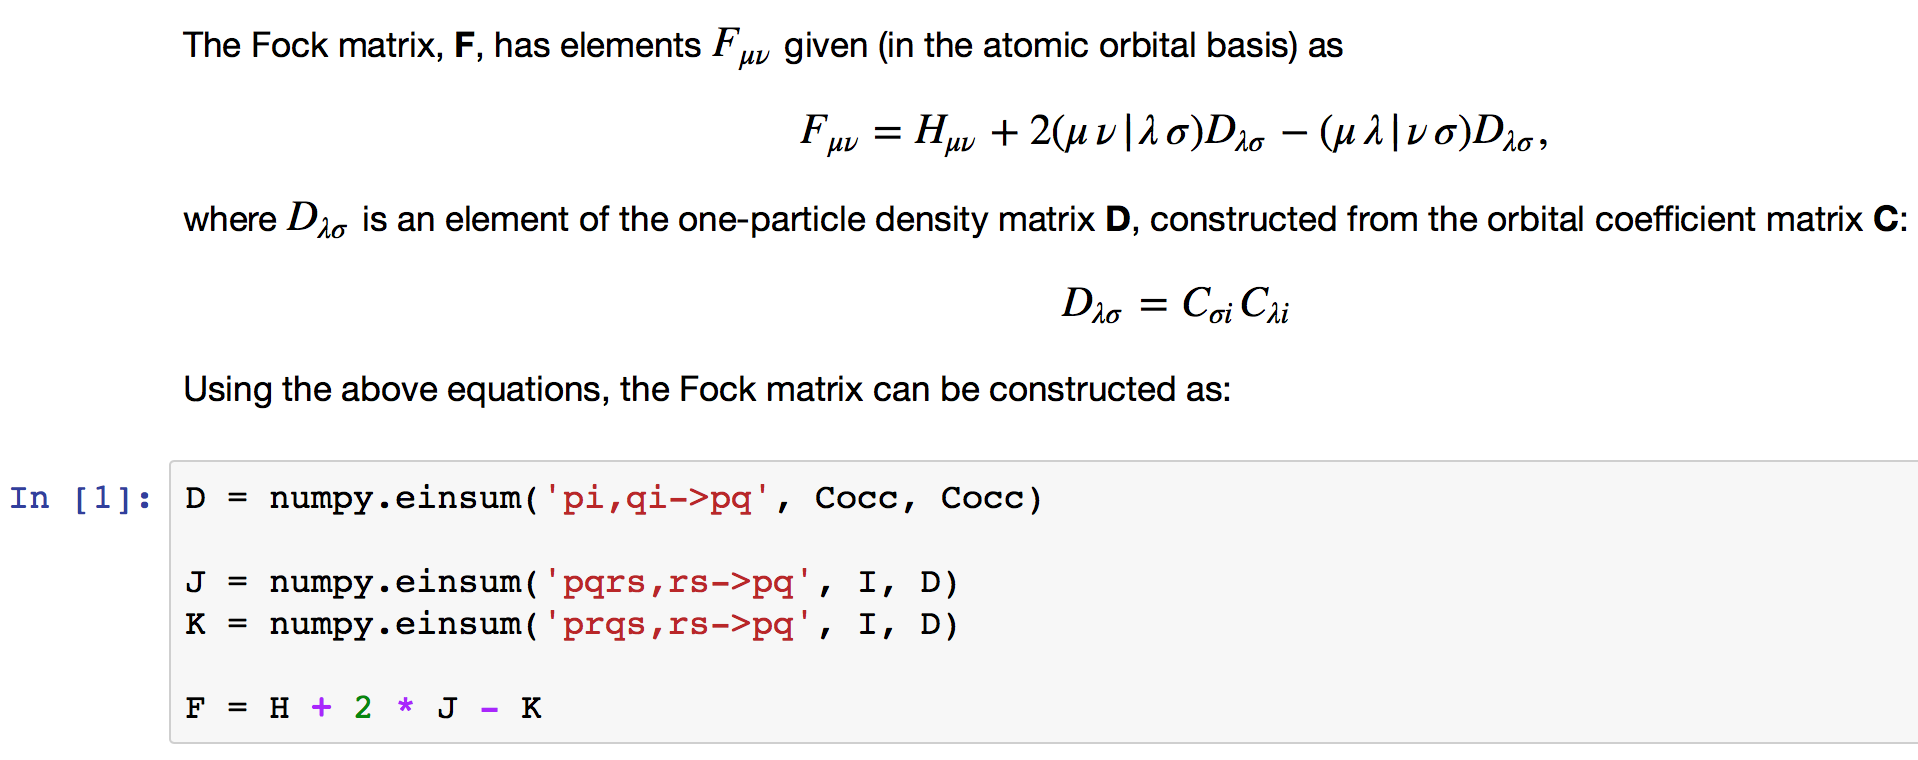
\includegraphics[width=\linewidth,keepaspectratio]{fig2-ipython-rhf.png}
  \caption{Extract from a Jupyter notebook demonstrating the construction of a SCF Fock matrix where {\tt I} is the 4-index electron repulsion integral array and {\tt Cocc} is the occupied orbital matrix.}
  \label{fig:ipython}
\end{figure}

These documents may be unique within quantum chemistry in that they focus not only on theoretical considerations but also on the details of a method's implementation, such as {\em why} certain programming choices were made. For example, the comparison between a general matrix inversion and solving a set of linear equations demonstrates instability issues that often plague the former technique. Such illustrations should make the Jupyter implementations useful both to new users in quantum chemistry and to experienced users interested in exploring new subfields.

% Whether a theorist wanting to learn or brush up on new quantum chemical methods or an instructor assembling a QC methods workshop, \pfn is a valuable resource. In particular, a learner is advised to read the introductory tutorial, \pfn Basics, then go directly to the implementation scripts, referring back to the later tutorials for enrichment, if needed.  An instructor will want to focus on the tutorials, perhaps devising exercises at the end of each for students to develop their syntax and method skills.

% Whether a student or enthusiast wanting to learn or brush up on quantum chemical methods, a prospective developer seeking good practices for manipulating \pfour's powerful C++ backend, an instructor assembling a QC methods or \pfour users workshop, or a researcher in need of a reference implementation validation, \pfn is a valuable resource. In particular, a learner is advised to read the introductory tutorial, \pfn Basics, then go directly to the implementation scripts, referring back to the later tutorials for enrichment, if needed. A developer should start with a familiar method, then examine all the variations and implementations to see how it's expressed for \pfour. An instructor (unless for an advanced workshop) will want to focus on the tutorials, perhaps devising exercises at the end of each for students to develop their syntax and method skills. A researcher whose target method is lodged with \pfn will naturally focus on adding variations to that script, validating his own code against them, and hopefully contributing his improvements back to \pfn.

Current tutorial-style Jupyter reference implementations include

\begin{enumerate}
\item Introductions to the \pfn methodology
\item Introduction to Hartree--Fock, DIIS, and density fitting
\item Density Functional Theory: grids, LDA kernels, VV10 dispersion, and asymptotic corrections
\item M\o ller--Plesset: canonical and density-fitted reference implementations of MP2
\item Molecular Properties: Integrals, CPHF, CIS
\item Symmetry-Adapted Perturbation Theory: Canonical and atomic orbital algorithms
\item Orbital-Optimized Methods: OMP2
\item Coupled-Cluster Approximations: CEPA0, CCD
\item  Geometry Optimization Techniques: Internal Coordinates, Hessian guesses, and advanced Newton-Raphson methods
\end{enumerate}
Molecular-dynamics tutorials include
\begin{enumerate}
\item Periodic Lennard-Jones simulation with Verlet integrators
\item Periodic Ewald Electostatic summation
\end{enumerate}

\section{Conclusions}

We believe that the benefits of the \pfn framework to the computational chemistry community are threefold.  Beginning researchers can use the \pfn reference implementations for {\em education}. Reference implementations convey not just the underlying mathematical formulas of a given theory, but how to implement these formulas in a manner that avoids common pitfalls such as ill-conditioned numerical equations. \pfn is likely the most interactive educational resource available in this field: thanks to the Jupyter Notebook format, the learners can explore the implementation step by step and easily try out various modifications and additional approximations.

More advanced researchers who need to reimplement and/or modify a given computational chemistry approach can use the \pfn reference implementations for {\em validation}, taking advantage of the code that, thanks to the extensive use of the \numpy \texttt{einsum} functionality, provides a nearly one-to-one correspondence between the terms in a formula and the lines of Python code. As a result, it is trivial to switch off, for debugging purposes, any subset of terms as well as generate an arbitrary intermediate without even recompiling any code.  This feature should be contrasted with the situation when one tries to validate their code against a C++/Fortran implementation from an established electronic-structure package. Once the relevant fragment of code that does the actual computation is found (which is not always trivial), various terms are typically combined in nontrivial ways to improve computational performance. As a result, getting out a specific intermediate for checking the implementation in progress often requires substantive changes to the reference code, not to mention its recompilation.  In addition, we include the programmed formulas together with their implementation in the Jupyter Notebook to alleviate difficulties associated with incompatible notation or even errors in the originally published expressions.

Finally, for researchers who want to develop new functionality, \pfn is a highly valuable platform for {\em initial implementation} that is efficient enough for meaningful testing, quick to generate, easy to debug, and has few opportunities for programming errors. All underlying quantum-chemistry building blocks such as integrals, orbitals, density matrices, and CI vectors are efficiently computed by \pfour and readily imported in the \numpy format. In particular, a \pfn implementation of any one-electron theory such as HF or DFT is already close to optimal as the most expensive operations are all written in terms of generalized Coulomb and exchange matrices which are supplied by \pfour.  Some of us, together with their collaborators, have already taken advantage of the \pfn capabilities to rapidly generate pilot implementations of brand new electronic-structure approaches.
% End Konrad's fragment here

\section{Associated Content\label{sec:si}}
Documents reproducing all currently available reference implementations and interactive tutorials are available free of charge via the Internet at \url{https://zenodo.org/record/1134320}. For all future materials, please see \url{https://github.com/psi4/psi4numpy}.

\section{Acknowledgements}
This work was supported in part by the U.S.~National Science Foundation through grants ACI-1449723 and CHE-1566192 for D.G.A.S, L.A.B., D.A.S, and C.D.S; CHE-1661604 for B.Z., A.S.A, J.M.T., and H.F.S; CHE-1554354 for D.R.N and A.E.D. B. Z. contributions to this work were also supported by a Software Fellowship from the Molecular Sciences Software Institute, which is funded by the U.S. National Science Foundation (ACI-1547580).  M.H.L. acknowledges financial support by the Studienstiftung des Deutschen Volkes. K.P.  is supported by the U.S. National Science Foundation CAREER award CHE-1351978.

\newpage
\bibliography{psi4numpy}

\end{document}
